\documentclass[landscape,usenames,dvipsnames]{sciposter}
\renewcommand{\papertype}{custom}
\renewcommand{\sectionsize}{\large}


% edit pointsize, width, height, and fontsize parameters as needed
% DO ensure that values in the \special commands match!
\usepackage[pass,paperwidth=36in,paperheight=24in]{geometry}
\renewcommand{\fontpointsize}{25pt}
\setmargins[2.5cm]

%\renewcommand{\subsectionsize}{\large \textcolor{\SectionCol}}
%\usepackage[spanish]{babel}
% or whatever
\usepackage{tikz}
\usetikzlibrary{arrows,automata,positioning}
\usepackage[latin1]{inputenc}
\usepackage{amsmath,amsthm,amssymb,bm}
\usepackage{multicol}
\usepackage{listings}
\usepackage{enumerate, wrapfig}
\usepackage{colortbl}
\usepackage[absolute]{textpos}
%\usepackage{subfigure}

\usepackage{graphicx}
\graphicspath{ {images/} }

%\newcommand{\reed}[1]{\relax}
%\newcommand{\abdullah}[1]{\relax}
%\newcommand{\tatum}[1]{\relax}
%\newcommand{\eric}[1]{\relax}
%\newcommand{\christian}[1]{\relax}
%\newcommand{\Fix}[1]{\relax}
\newcommand{\reed}[1]{{\color{magenta}\bfseries [#1]}}
\newcommand{\abdullah}[1]{{\color{blue}\bfseries [#1]}}
\newcommand{\tatum}[1]{{\color{orange}\bfseries [#1]}}
\newcommand{\eric}[1]{{\color{green}\bfseries [#1]}}
\newcommand{\christian}[1]{{\color{cyan}\bfseries [#1]}}
\newcommand{\Fix}[1]{{\color{red}\bfseries [#1]}}
\newcommand{\Comment}[1]{}
\newcommand{\Space}[1]{}
\newcommand{\Num}[1]{#1}

\newcommand{\term}[1]{\emph{\textbf{#1}}}

\newcommand{\R}{\mathbb{R}}
\newcommand{\Q}{\mathbb{Q}}
\newcommand{\Z}{\mathbb{Z}}
\newcommand{\N}{\mathbb{N}}

\theoremstyle{definition}
\newtheorem{definition}{Definition}[section]
\theoremstyle{remark}
\newtheorem{remark}[definition]{Remark}
\theoremstyle{remark}
\newtheorem{example}[definition]{Example}
\theoremstyle{plain}
\newtheorem{theorem}[definition]{Theorem}
\newtheorem{conjecture}[definition]{Conjecture}

\lstdefinelanguage{pecan}{
	keywords=[1]{forall, exists, max, min, sup, inf, are, is, if, then, match, with, case, end, let, be, in, else, iff},
	keywordstyle=[1]\color{blue}\bfseries,
	keywords=[2]{false, true, sometimes},
	commentstyle=\color{CadetBlue}\textit,
	stringstyle=\color{ForestGreen}, % string literal style
	keywordstyle=[2]\color{orange}\bfseries,
	keywords=[3]{assert_prop,Structure,defining,Theorem,Prove,Example,Alias,Restrict,Define,Display,Execute,load,shuffle,import,save_aut,save_aut_img,that,context,end_context,forget,shuffle,shuffle_or,using,of},
	keywordstyle=[3]\color{teal}\bfseries,
	keywords=[4]{@annotation,@postprocess,@no_simplify,@simplify,@simplify_states,@simplify_edges},
	keywordstyle=[4]\color{purple}\bfseries,
	literate=%
	    {\#}{{{\color{teal}\bfseries\#}}}1
	    {+}{{{\color{red}+~}}}1
	    {-}{{{\color{red}-~}}}1
        {:=}{{{\color{red}:=~}}}1
        {..}{{{\color{red}..~}}}1
        {\{}{{{\color{red}\{}}}1
        {\}}{{{\color{red}\}}}}1
        {|}{{{$\color{red} \lor~$}}}1
        {*}{{{\color{red}*~}}}1
        {:}{{{\color{red}:~}}}1
        {>}{{{\color{red}>~}}}1
        {<}{{{\color{red}<~}}}1
        {<=>}{{{$\color{red}\Leftrightarrow~$}}}1
        % <= conflicts with <=> as iff, so I commented it out because it's more importnat that <=> not look weird (it becomes \leq > with the following line).
        % But might as well keep something, so I keep \iff
        % {<=}{{{$\color{red} \leq$}}}1
        % Also got rid of >= for consistency.
        % {>=}{{{$\color{red} \geq$}}}1
        {.}{{{\color{red}.~}}}1
        {&}{{{$\color{red} \land~$}}}1
        {!}{{{$\color{red}\lnot~$}}}1
        {!=}{{{$\color{red} \neq$}}}1
        {=}{{{\color{red}=~}}}1
        {exists }{{{$\color{red}\exists$}}}1
        {forall }{{{$\color{red}\forall$}}}1,
    sensitive=false, % keywords are not case-sensitive
    morecomment=[l]{//}, % l is for line comment
    morecomment=[s]{/*}{*/}, % s is for start and end delimiter
    morestring=[b]", % defines that strings are enclosed in double quotes
    showstringspaces=false
}

\lstnewenvironment{pecan}
  {
    \lstset{
        language=pecan, 
        basicstyle=\small\ttfamily, 
        mathescape=true
        }
  }
  {
  }

\lstnewenvironment{pecan_output}
  {
    \lstset{
        basicstyle=\small\ttfamily,
        mathescape=true
        }
  }
  {
  }

\newcommand{\pecaninline}[1]{\lstinline[language=pecan,basicstyle=\small\ttfamily,mathescape]{#1}}


\newtheorem{thm}{Theorem}%[section] % uncomment [section] to number within section
\newtheorem*{thm*}{Theorem}
\newtheorem{lem}{Lemma}
\newtheorem{cor}[thm]{Corollary}
\newtheorem{prop}[thm]{Proposition}
\newtheorem{rem}[thm]{Remark}
\newtheorem{cond}[thm]{Condition}
\newtheorem*{namedtheorem}{Theorem}
\newtheorem*{ex}{Example}
\newtheorem*{defin}{Definition}
\newtheorem{env}[thm]{Variation}
\renewcommand {\theequation}{\arabic{section}.\arabic{equation}}

%Lines 54-73 define box theorem. You can do similar things to put boxes around conjectures, corollaries, ect, or use the mdframe to just create a box
\usepackage[framemethod=TikZ]{mdframed}
\definecolor{light-blue}{RGB}{197,219,249}
\mdfdefinestyle{MyFrame}{linecolor=light-blue,
    outerlinewidth=1.5pt,
    roundcorner=0pt,
    innertopmargin=7pt,
    innerbottommargin=7pt,
    innerrightmargin=15pt,
    innerleftmargin=15pt,
    backgroundcolor=light-blue}
\mdfdefinestyle{thmsytle}{linecolor=orange,
    outerlinewidth=2pt,
    roundcorner=20pt,
    innertopmargin=15pt,
    innerbottommargin=15pt,
    innerrightmargin=15pt,
    innerleftmargin=15pt,
    backgroundcolor=white,
	}


\mdtheorem[style=thmsytle]{MDtheorem}{Theorem}
\newcommand*{\Title}{}
\newenvironment{boxthm}[1][]{%
\refstepcounter{thm}
    \ifstrempty{#1}{\begin{MDtheorem}}%
    {\begin{MDtheorem}[(#1)]}
}{%
    \end{MDtheorem}%
}%

%%hyperlinks
\usepackage{hyperref}
 
% \usepackage[
% backend=biber,
% style=alphabetic,
% sorting=ynt
% ]{biblatex}

% \addbibresource{bibliography.bib}


%\definecolor{BoxCol}{rgb}{0.9,0.9,0.9}
% uncomment for grey background to \section boxes
% for use with default option boxedsections

\definecolor{BoxCol}{rgb}{.06,.16,.28}


\definecolor{SectionCol}{rgb}{1,1,1}

\definecolor{blue}{rgb}{0,0,1}
\definecolor{orange}{rgb}{.93,.29,0.1}
\definecolor{white}{rgb}{1,1,1}

\newtheorem{Features}{Features}

\title{Automatic Theorem Proving}

\author{
Authors: Reed Oei, Eric Ma, Tatum Schmidt, Abdullah Dean \\
Graduate Mentor: Christian Schulz \\
Faculty Advisor: Philipp Hieronymi \\
}

%\institute{University of Illinois at Urbana-Champaign}
%\email{}  shows author email address below institute

%\date is unused by the current \maketitle

%%%%%%%%%%%%%%%%%%%%%%%
% Logo for Poster
%%%%%%%%%%%%%%%%%%%%%

\leftlogo[.7]{igl-logo-small.png} % defines logo to left of title (with scale factor)
\rightlogo[.6]{imark.png} % same but on right

%%%%%%%%%%%%%%%%%%%
% Start of document
%%%%%%%%%%%%%%%%%%%
\begin{document}
%%%%%%%%%%%%%%%%%%%%%%
%% Poster Set up
%%%%%%%%%%%%%%%%%%%%%%%
% \conference{Undergraduate Research Symposium SP 2020}
\conference{IGL Poster Session Spring 2020}

\maketitle
\vspace{-3ex}
\begin{multicols}{3}  % sets up 3 column poster



%%%%%%%%%%%%%%%%%%%%%%
%% Start of First Column
%%%%%%%%%%%%%%%%%%%%%%%
\section*{Introduction}
% \begin{mdframed}[style=MyFrame]
% \subsection*{Automated Theorem Proving}
% \end{mdframed}

An \textbf{automated theorem prover} is a program that takes a statement and \emph{decides} (i.e., proves or disproves) it. 
Theorem provers can be very useful: computers are reliable, and they never get tired or bored, allowing us to quickly explore new ideas.
Though it is impossible to decide \emph{all} statements, we can still use theorem provers to solve many interesting problems. 

%%%%%%%%%%%%%%%%%%%%%%%%%%%%%%%%%%%%%
%% Pecan
%%%%%%%%%%%%%%%%%%%%%%%%%%%%%%%%%%%%%
\section*{Pecan: A Theorem Prover}

\textbf{Pecan} is a system we are developing for automated theorem proving that represents logical predicates using B\"uchi automata.
Pecan programs are made up of \textbf{predicates} and \textbf{directives}:

\begin{itemize}
    \item predicates: defined either by loading automata defined in files, translating LTL (linear temporal logic) formulas into B\"uchi automata, or some combination of these using first order logic and equality.

\begin{pecan}
y is successor_of(x) := x < y & forallz. z <= x | y <= z
\end{pecan}

    \item directives: commands to the Pecan interpreter, such as: \pecaninline{Theorem}, which asks Pecan to prove a theorem, or \pecaninline{save_aut}, which asks Pecan to build the automaton corresponding to some predicate and save it to a file

\begin{pecan}
Theorem ("Equality is symmetric.", { forallx,y. x = y iff y = x }).
\end{pecan}

\end{itemize}

% The Pecan language is a statically-typed and interpreted.
% The basic datatype, or universal set, in Pecan is the infinite binary word---elements of $\Sigma^{\omega}$ where $\Sigma = \{0,1\}$.
% All types are \textbf{refinement types}: they define a subset of $\Sigma^{\omega}$ satisfying some predicate defined using B\"uchi automata.

% \begin{ex}
% A word $x \in \Sigma^\omega$ has type \texttt{binary} if $x \in \{ w \in \Sigma^* : x = w0^\omega \}$---that is, binary words that are eventually $0$.

% Equivalently, we can define $\texttt{binary}$ as the words satisfying the LTL formula $\lozenge \square \lnot x$.
% \end{ex}

% Users can define their own \textbf{structures} on a type so that names can be overloaded: for example, this allows users to define their own numeration systems.

% \begin{lstlisting}[language=pecan, basicstyle=\normalsize\ttfamily, mathescape=true, frame=single]
% Structure binary defining {
%     "adder": bin_add(any, any, any),
%     "less": bin_less(any, any) 
% }
% \end{lstlisting}

Pecan is capable of proving any statement expressed solely in terms of B\"uchi automata and first order logic connectives, such as $\wedge$, $\vee$, $\neg$, $\forall$, and $\exists$.
In particular, Pecan is powerful enough to decide any statement in Presburger arithmetic, the first order theory of the natural numbers with addition (but \emph{not} multiplication by variables) and comparison.
Try out Pecan at \url{http://reedoei.com/pecan}.

\section*{The Chicken McNugget Problem}

% In the 1980s, Henri Picciotto asked the following problem in his algebra textbook:

\begin{quote}
    What is the greatest number of chicken nuggets that cannot be ordered using only boxes of 6, 9, and 20?
\end{quote}

We call all such numbers \textbf{non-purchasable}, and we can define them in Pecan as follows:

\begin{lstlisting}[language=pecan, basicstyle=\normalsize\ttfamily, mathescape=true, frame=single]
Restrict n,m,a,b,c are binary.
n is purchasable := n is binary & existsa,b,c. n =$\ $6*a $\color{red} +$ 9*b $\color{red} +$ 20*c
n is non_purchasable := n is binary & !(n is purchasable)
\end{lstlisting}

We can then define the largest non-purchasable number naturally as:
\begin{lstlisting}[language=pecan, basicstyle=\normalsize\ttfamily, mathescape=true, frame=single]
largest(n) := n is non_purchasable & 
              forallm. if m is non_purchasable then n >= m
\end{lstlisting}

\begin{figure}
    \centering
    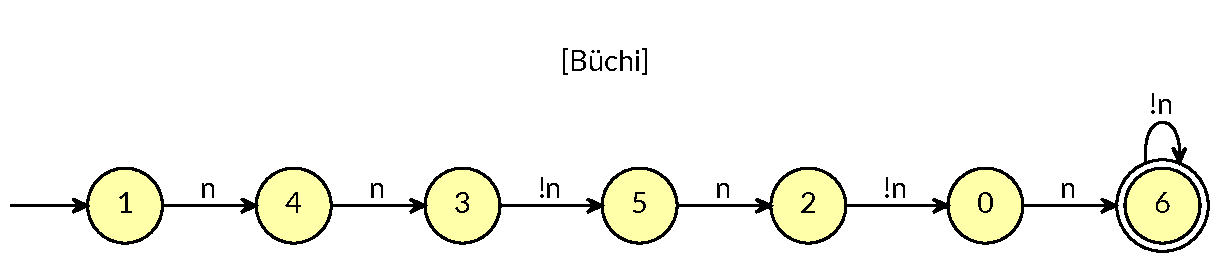
\includegraphics[width=\textwidth]{images/largest_not_purchasable.pdf}
    \caption{The B\"uchi automaton representing \pecaninline{largest(n)}, which accepts $110101_2$ ($43$ in base 10) in least significant digit first representation.}
    \label{fig:largest_non_purchasable}
\end{figure}

We can also ask Pecan to show us what numbers \pecaninline{largest} accepts, and it will automatically perform the necessary conversions.
\begin{pecan}
Example (natFormat, { largest(n) }). // Prints [(n,43)]
\end{pecan}

\columnbreak

\section*{The Thue-Morse Word}

We now turn to \textbf{automatic sequences}, words defined by automata, starting with the Thue-Morse word, $T$. 
The $n$-th digit of the Thue-Morse word, $T[n]$, is $1$ if the binary representation of $n$ has an odd number of $1$'s, and $0$ otherwise.
The Thue-Morse word starts with: $01101001100101101001011001101001\ldots$

\begin{defin}
    A word $w$ is a \textbf{square} if it is of the form $w = xx$ for some word $x$.
    Similarly, $w$ is a \textbf{cube} if it is of the form $w = xxx$ for some word $x$.
\end{defin}

\begin{mdframed}[style=MyFrame]
\begin{thm}
    The Thue-Morse word does not contain any cubes.
\end{thm}
\end{mdframed}

Below is a Pecan definition of cubes in the Thue-Morse word and the theorem we would like to prove.
\begin{lstlisting}[language=pecan, basicstyle=\normalsize\ttfamily, mathescape=true, frame=single]
Restrict i,j,n are binary.
square(i, n) := n > 0 & T[i..i+n] = T[i+n..i+2*n]
cube(i,n) := square(i, n) & square(i+n, n)
Theorem ("T does not contain cubes", { !(existsi,n. cube(i,n)) }).
\end{lstlisting}

\begin{lstlisting}[basicstyle=\normalsize\ttfamily, mathescape=true, frame=single]
[INFO] Checking if T does not contain cubes is true.
$\color{ForestGreen} \text{T does not contain cubes is true.}$
\end{lstlisting}

\begin{mdframed}[style=MyFrame]
\begin{thm}
There are no overlapping squares, i.e., words of form $0x0x0$ or $1x1x1$ for some nonempty word $x$. 
\end{thm}
\end{mdframed}

We can check it by running the following Pecan commands.

\begin{lstlisting}[language=pecan, basicstyle=\normalsize\ttfamily, mathescape=true, frame=single]
Theorem ("T does not contain overlapping squares.", 
    { !(existsi,n. n > 0 & square(i,n) & T[i] = T[i+2*n]) }).
\end{lstlisting}
Pecan verifies the theorem: 
\begin{lstlisting}[basicstyle=\normalsize\ttfamily, mathescape=true, frame=single]
[INFO] Checking if T does not contain overlapping squares is true.
$\color{ForestGreen} \text{T does not contain overlapping squares is true.}$
\end{lstlisting}

%%%%%%%%%%%%%%%%%%%%%%%%%%%%%%%%%%%%%
%% New Section
%%%%%%%%%%%%%%%%%%%%%%%%%%%%%%%%%%%%%
\section*{Characteristic Sturmian Words}
A \textbf{cutting sequence} for a curve is a sequence of $0$'s and $1$'s, corresponding to when the line crosses vertical and horizontal grid lines, respectively.
\textbf{Characteristic Sturmian words} are infinite binary sequences defined by the cutting sequence of $y = \alpha x$ for some irrational $\alpha \in (0,1)$ in the Cartesian plane.
Figure~\ref{fig:fib_word} shows the characteristic Sturmian word with slope $\frac{1}{\phi}$, which begins $0100101001\ldots$.

\centerline{
\begin{minipage}{.6\columnwidth}
%Insert Picture of automaton
\begin{figure}
	\centering
    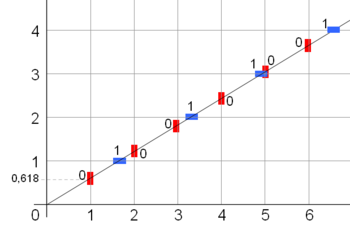
\includegraphics[width=0.8\columnwidth]{images/Fibonacci_word_cutting_sequence.png}
    \caption{Characteristic Sturmian word with slope $\frac{1}{\phi}$}
    \label{fig:fib_word}
\end{figure}
\end{minipage}
}

Sturmian words are \textbf{automatic sequences} meaning that there are automata which calculate their $n$-th digit given the number $n$ in special numeration systems called \textbf{Ostrowski numeration systems}.
With the addition automaton for general Ostrowski numeration systems, we are able to use Pecan to \emph{automatically prove} properties about Sturmian words. 
% as those in Du, Mousavi, Schaeffer, and Shallit's paper "Decision Algorithms for Fibonacci-Automatic Words, with Applications to Pattern Avoidance" for the \textbf{characteristic Sturmian word with all slopes} instead of for the original Fibonacci word.
% \vspace*{0.4em}

% \begin{definition}
% The \textbf{characteristic Sturmian word with slope $\sqrt[~]{2}$}, which we denote as $C_2$, is the infinite word obtained as the limit of the sequence of \textbf{standard words} $s_n$ defined by{
% \setlength{\abovedisplayskip}{3pt}
% \setlength{\belowdisplayskip}{3pt}
% $$ s_n=s^{d_n}_{n-1}s_{n-2} \text{ when } n\ge 2, \text{ where } s_1= 0^{d_1-1}1 \text{ and } s_0=0.$$}
% \end{definition}
% By having built the Ostrowski-$\sqrt[~]{2}$ numeration system and the automatic word $C_2$ in Walnut, we may use the command $C2[i]$ to return the $i^{th}$ digit of $C_2$.\\

\columnbreak

\section*{Theorems about Sturmian Words}

There are many interesting properties of Sturmian words, and we can use Pecan to automatically prove many of these.

\begin{defin}
    A word is eventually periodic if it is of the form $abbbbb \ldots$ for some subwords $a$ and $b$ (e.g., $0.1024545454545\ldots$ where the repeating part is $45$).
\end{defin}

\begin{mdframed}[style=MyFrame]
\begin{thm}
Sturmian words are not eventually periodic.
\end{thm}
\end{mdframed}
\begin{proof}
In Pecan, we can write this statement as:

\begin{pecan}
eventually_periodic(a, p) := 
    p > 0 & existsn. foralli. if i > n then C[i] = C[i+p]
Theorem ("Sturmian words are not eventually periodic", 
{ foralla,p. if p > 0 then !eventually_periodic(a,p) }).
\end{pecan}

The automata have hundreds of states, and its nearly impossible to understand them by looking at pictures of them.
\end{proof}

\begin{defin}
    A word is a palindrome if reversing it gives the same word (e.g., ``racecar'' or ``0110'').
\end{defin}

\begin{mdframed}[style=MyFrame]
\begin{thm}
All Sturmian words contain palindromes of every length $n$; furthermore, if $n$ is even then there is exactly one palindrome, and if $n$ is odd there are exactly two.
\end{thm}
\end{mdframed}

\begin{proof}
Using Pecan, we first define a palindrome, then we define the first occurrence of each palindrome, giving us a unique position for each palindrome of each length, and finally we ask Pecan to prove the theorem.
\begin{pecan}
palindrome(a,i,n) :=
    forallt. if t < n then C[i + t] = C[i+n-1-t]
first_palindrome(a,i,n) := palindrome(a,i,n) & 
    forallj. if j > 0 & C[j..j+n] = C[i..i+n] then i <= j
\end{pecan}
    
Finally, we state the theorem and ask Pecan to prove it.
\begin{pecan}
Prove that { foralla,n. (
if n is even then 
    existsi. forallj. first_palindrome(a,j,n) iff i=j
) & (
if n is odd then
    existsi,j. i!=j & forallk. first_palindrome(a,k,n) iff (i=k | j=k)
)}.
\end{pecan}
\end{proof}

These examples highlight Pecan's ability to quantifying over uncountable sets of strings, something that previous theorem provers with a similar approach, such as Walnut, were unable to do.
This allows us to state and prove theorems about \emph{all} Sturmian words, instead of just individual Sturmian words.

\section*{Future Work}
\begin{itemize}
\item Continue to develop Pecan.
\item Write a paper about Pecan and the various properties of Sturmian words we are able to automatically prove.
\item Since Pecan uses B\"uchi automata, which accept infinite words, we can represent sets of real numbers using B\"uchi automata and prove properties about the real numbers.
\end{itemize}

% \vspace*{-10pt}  %change to -10
\section*{References}

{\footnotesize [1] Khoussainov, Bakhadyr.Nerode, Anil. (2001) \emph{Automata Theory and its Applications}, MA : Birkh\"auser Boston
}

{\footnotesize [2] Hamoon Mousavi. \emph{Automatic Theorem Proving in Walnut}. In: CoRR abs/1603.06017 (2016).
arXiv: 1603.06017. url: http://arxiv.org/abs/1603.06017.
}

{\footnotesize [3] Du, Chen Fei. Mousavi, Hammoon. Schaeffer, Luke and Shallit, Jeffrey. (2014) \emph{Decision Algorithms for Fibonacci-Automatic Words, with Applications to Pattern Avoidance}
}

{\footnotesize [4] Hieronymi, P., \& Terry Jr, A. (2018). \emph{Ostrowski Numeration Systems, Addition, and Finite Automata}. Notre Dame Journal of Formal Logic, 59(2), 215-232.
}

\vspace*{10mm} %This will change to -5
\emph{
Support for this project was provided by the Illinois Geometry Lab and the Department of Mathematics at the University of Illinois at Urbana-Champaign.
}
\end{multicols}

\end{document}
